% -*-LaTeX-*-

% $Log: audio-video.tex,v $
% Revision 1.4  2007/03/20 22:43:09  stiber
% Revised for stand-alone textbook.
%
% Revision 1.3  2006/03/27 23:40:41  stiber
% Fixed minor typos.
%
% Revision 1.2  2004/03/29 19:49:39  stiber
% Updated for Spring 2004 and new textbook (DSP First).
%
% Revision 1.1  2004/02/19 00:27:44  stiber
% Initial revision
%

\chapter{Audio \& Video Compression and Coding}
\label{ch:audio-video}

This chapter continues our coverage of compression begun in
chapter~\ref{ch:compression} with descriptions of current standard
compression schemes for audio and video information.  By the end of
this chapter, you will have a basic understanding of how the most
common compression and coding algorithms use the fundamentals of
lossless and lossy compression. You will also understand how the
nature of the multimedia application influences compression algorithm
design.

Each coding algorithm or standard discussed in this chapter
shows clearly the tradeoffs inherent in lossy versus lossless
compression, the need for symmetric coding and decoding versus the
ability to asymmetrically place more processing power in the encoder,
storage versus transmission, and human perception versus machine
processing. We begin with audio coding schemes, move on to those
for still images, and conclude with video.

More specifically, each coding scheme makes implicit or explicit
decisions about each of the following issues; you should consider
what those decisions are when you read about each standard.

\subsection{Issues in Coding Method Selection}
\begin{itemize}
\item What are the application constraints? Are there signal quality
requirements? Limits on system complexity? Upper bounds on end-to-end
transmission delay?
\item Will the codec (CODer/DECoder) be implemented in software,
hardware, or a hybrid combination of both?
\item Should the encoding be reversible, or can it be lossy?
\item Besides overall constraints on algorithm efficiency, are there
constraints on efficiency \emph{consistency}? In other words, can the
amount of computation required vary (based on the time-varying nature
of the signal), or must it be independent of the signal's content?
\item Does the algorithm need to be tolerant of transmission errors?
Does it need to be able to correct them? How should it deal with data
lost in transmission?
\item If a lossy algorithm is desired, what kind of information can be 
lost? How do we decide what information to throw away?
\item Does the data representation need to accommodate future
scalability?  For example, are we building a codec for images up to
some maximum size, or will we want it to work with larger images in
the future?
\item How many times will the media be encoded? Decoded?
\item Will we need to synchronize the encoded signal with other media, 
or are we encoding it ``in isolation''?
\item Will our system need to be compatible with other methods?  Will
we need to ``transcode'' our representation to other formats, or
transcode other formats to our representation, efficiently?
\end{itemize}

\section{Audio Coding Standards}

\subsection{Speech Coding for Telephony}

Pulse code modulation (PCM), as discussed in
chapter~\ref{ch:compression}, is the foundation for most of the major
audio coding standards. The ITU (International Telecommunications
Union) has defined the following audio coding standards (among others)
for ``low quality'' (i.e., telephone quality) audio:

\begin{description}
\item[G.711] This is audio pulse-code modulation (PCM) in support of video
conferencing, with a bandwidth of 64K bits/second.  It recommends a
sampling rate of 8000 samples/second.  The audio data is
logarithmically encoded (which has the effect of companding) to 8
bits, quantized to 212 levels. The encoding itself can be either A-law
(this is mostly used in Europe) or $\mu$-law (which is mostly used in
the US and by most computer hardware and software).
\item[G.721] This is an ADPCM-based standard for 32K bit/second audio.
\item[G.726] This replaces G.721, allowing conversion between 64Kbps
and 40, 32, 24, or 16kbps.
\item[G.727] This standard extends G.726 for embedded applications,
including transmission over packet-switching networks (packetized
voice protocol, or PVP, which is G.764).
\item[G.722 and G.725] These standards are targeted at higher-quality
speech transmission, with a signal bandwidth of 50Hz to 7kHz. They are
targeted at a transmission rate of 64kbps.
\end{description}

There are other approaches that aim to produce high-quality speech
with low bandwidth requirements (below 16kbps). These include LPC
(linear predictive coding) and CELP (code excited linear
predictor). In both cases, a model of the speaker's vocal tract is
generated and the parameters of this model are transmitted to the
receiver. After that, only enough data is sent to allow for the
\index{compression!speech synthesis and}
receiver to \emph{synthesize} speech using the model. So, instead of
hearing a processed version of the speaker's voice, the listener hears
a synthesized approximation to their voice. To improve speech quality, 
CELP sends error information (the difference between the actual signal 
and the model's output) in addition to the model information.

\subsection{High-Quality Audio Coding}

There are a number of standards used to encode audio at quality levels 
usable for music, television, movies, etc. --- up to audiophile levels 
(except perhaps for those folks who insist that tube amplifiers and
vinyl are necessary to capture the warmth of the original music).  

\subsubsection{MPEG}

While MPEG (Moving Picture Experts Group) is a standard for video
encoding, it obviously also must include audio information and is
often used in isolation for just encoding audio. MPEG is actually a
family of standards, with successive members providing increased
quality at higher levels of compression (at the price of increasing
computational complexity). For almost all versions, the input signal
is assumed to be 20kHz. (What is the minimum sampling rate for such a
signal [answer in~\ref{sc:ch9ex}
\#\ref{it:ch9ex1}]?) The desire is to have quality
comparable to compact disc audio, and to support multiple channels of
such audio. For CD quality, at a sampling rate of 44.1kHz, 16
bits/channel and two stereo channels, the uncompressed audio stream is 
1.4Mbps.

\paragraph*{MPEG-I}
This standard allows for encoding of two channels (stereo) at sampling
rates of 32 (FM broadcasting), 44.1 (CD), or 48 (DAT) kHz. It achieves
high-quality lossy compression by incorporating a simple
psychoacoustical model of human auditory perception. The algorithm
\index{perception!auditory}
\index{psychoacoustics}
uses this model to determine what information can be lost without
significantly affecting the listener's perception of sound quality.

More specifically, the algorithm is based on the phenomenon called
\emph{masking}. It is perhaps not surprising that our auditory systems 
are not equally sensitive to all sound frequencies.  We are most
sensitive to sounds in the range of 2--4kHz, and increasingly less
sensitive to much higher and lower frequencies. What might be
surprising is that our sensitivity at one frequency can be influenced
by the presence of sounds at other frequencies.

The general idea of masking is that signals can interfere with each
other within the processing stages that are a part of sensory
systems. For example, a signal at one frequency (a
\emph{masker}) presented around the same time as another one at a
second frequency might result in the second being undetected by the
sensory system.  This can occur even though the sensory system is
perfectly capable of perceiving the second signal in isolation (or, in
combination with signals other that the masker). Masking can also
occur in time (hence, my previous statement, ``around the same
time''), with our sensitivity to sound at some frequency recovering
from its masked level over the course of around 100ms.

In other words, how important a particular frequency is for our
perception of sound is a function of both the frequency itself
\emph{and} the history of signal intensities at other frequencies.

MPEG-I takes advantage of masking for compression by dynamically
altering a threshold for each of a number of frequency bands, based on
the signal strength in neighboring bands. It does this by passing the
input signal through a \emph{filter bank} composed of 32 bandpass
filters, thereby breaking the signal into 32 bands.  It then computes
the amount of masking for each band based on the signal in the other
bands.  The information in a band is only encoded if it is above the
masking threshold. If it is encoded, the number of bits to be used is
computed so that the quantization noise introduced is below the
masking threshold (remember the discussion of quantization noise in
chapter~\ref{ch:computer-signals}?). The resulting sub-band codes are
then formatted into a bitstream, perhaps with video and
synchronization information.

\begin{window}[3,r,%
\sidebar{\textbf{Web Links:}
\begin{description}
\item[Compression FAQ] \url{http://www.faqs.org/faqs/compression-faq/}
\item[JPEG image compression FAQ] \url{http://www.faqs.org/faqs/jpeg-faq/}
\item[Planet JPEG] \url{http://www.geocities.com/tapsemi/}
\item[MPEG section of compression FAQ]
  \url{http://www.faqs.org/faqs/compression-faq/part2/section-2.html}
\item[MPEG FAQ] \url{http://www.faqs.org/faqs/mpeg-faq/}
\item[MPEG.org] \url{http://www.mpeg.org/MPEG/index.html}
\begin{sloppypar}
\item[MPEG for MATLAB] \url{http://www.cl.cam.ac.uk/~fapp2/software/mpeg/}
\end{sloppypar}
\item[comp.compression newsgroup] \url{news:comp.compression}
\item[comp.multimedia newsgroup] \url{news:comp.multimedia}
\item[International Telecommunications Union (ITU)] \url{http://www.itu.int/}
\end{description}},{}]
MPEG-I actually includes three audio ``layers,'' each successive one
being an enhancement of the previous. Layer 1 uses bands of equal
width and only frequency masking (no temporal masking). Since it uses
only frequency masking, the codec only needs to keep one ``frame'' of
audio information (12 samples) in memory: masking occurs only between
bands at the current time. Layer 1 typically achieves compression
ratios of 4:1, or 384kbps high-quality stereo.

Layer 2 uses three frames of audio information in memory: previous,
current, and next.  This allows it to compute temporal masking, in
addition to frequency masking.  This allows layer 2 to reach
compression ratios of 8:1, for a 192kbps audio stream.

Layer 3 uses frequency bands which are not of equal width, to better
match human auditory perception.  It also seeks to eliminate
redundancy between the two stereo channels (because much of the
information in one channel is also present in the other). It does this
by separately coding the sum ($M$, for ``middle'') of the left ($L$)
and right ($R$) channels and their difference ($S$, for ``side'').  At
the decoder, the two channels are reconstructed as $L =
(M+S)/\sqrt{2}$ and $R = (M-S)/\sqrt{2}$. When you listen to an MP3
audio file, you are actually listening to MPEG-I, layer 3 encoded
audio. Finally, layer 3 incorporates Huffman coding for additional
data stream compression. Layer 3 can produce high-quality audio at a
compression rate of 12:1, which corresponds to a 112kbps data stream.
\end{window}

\paragraph*{MPEG-II}
This extends MPEG-I audio to five channels plus one additional,
low-frequency enhancement (LFE) channel. This should be familiar to
you as the basic configuration for surround-sound (the five channels
are center front, front left and right, and rear left and right; the
low-frequency channel is for a subwoofer).  These channels could also
be used to encode multilingual stereo.  The additional channels are
encoded by being mixed in such a way that an MPEG-I decoder can still
decode the primary left and right stereo channels from an MPEG-II
stream. So, an MPEG-II audio bit stream is an MPEG-I bit stream with
the additional data formatted into data blocks reserved in MPEG-I
for ancillary data. Correspondingly, an MPEG-II encoder consists of
an MPEG-I encoder and an MPEG-II extension encoder.

There are other implementations within the MPEG-II standard which are
not backward compatible with MPEG-I. These include AAC (advanced audio 
encoding).

\paragraph*{MPEG-III}
Because of the progress of MPEG-II in support of high-definition
television, development of an MPEG-III standard was terminated.

\paragraph*{MPEG-IV}
MPEG-IV is targeted at a much broader range of applications than the
preceding standards.  This includes not only compression and coding of 
audio and video, but support for structuring content for WWW and
hypermedia applications, intellectual property right management,
computer network quality of service signaling, interactivity by the
user, and low bit rate applications. It encodes data as a composition
of multimedia objects, which can include audio, video, and 3D
graphical objects.  This builds on the earlier work of VRML (virtual
reality modeling language). Little of this has anything directly to do 
with high-quality audio, but it seemed to make sense to discuss this
standard right after the other ones.

\section{Still Image Coding Standards}

There are a number of formats for single images. These include TIFF
(tag image file format) and GIF (graphics interchange format), which
are lossless formats that use Lempel-Ziv compression. Because it also
serves as the basis for spatial redundancy reduction in video, I'll
confine myself to discussing JPEG (Joint Photographic Experts Group).

\subsection{JPEG}

Actually, dismissing formats such as
TIFF and GIF was a bit misleading. Those are \emph{file formats}, while JPEG is an
\emph{encoding scheme}. In fact, JPEG-encoded images can be stored in
their ``own'' format (JFIF, for JPEG file interchange format) or
stored within a TIFF format file (which, counterintuitively, provides
greater flexibility and more advanced features).

JPEG is targeted at compression of continuous-tone color and grayscale
images (as opposed to line drawings). It includes a parameterized
encoder which can support four lossy or lossless modes. These modes
include:
\begin{description}
\item[Sequential] The image is encoded in a single top-to-bottom,
left-to-right scan.
\item[Progressive] The image is scanned multiple times, with
successive scans providing information for successively better
approximations to the original image.
\item[Lossless] Only entropy encoding is used.
\item[Hierarchical] Multiple versions of the image are encoded, at
successively finer resolution. This allows a receiver to select the
appropriate resolution; the encoder needn't know the limitations of
the decoder or the constraints of its application.
\end{description}

\begin{figure}
\centerline{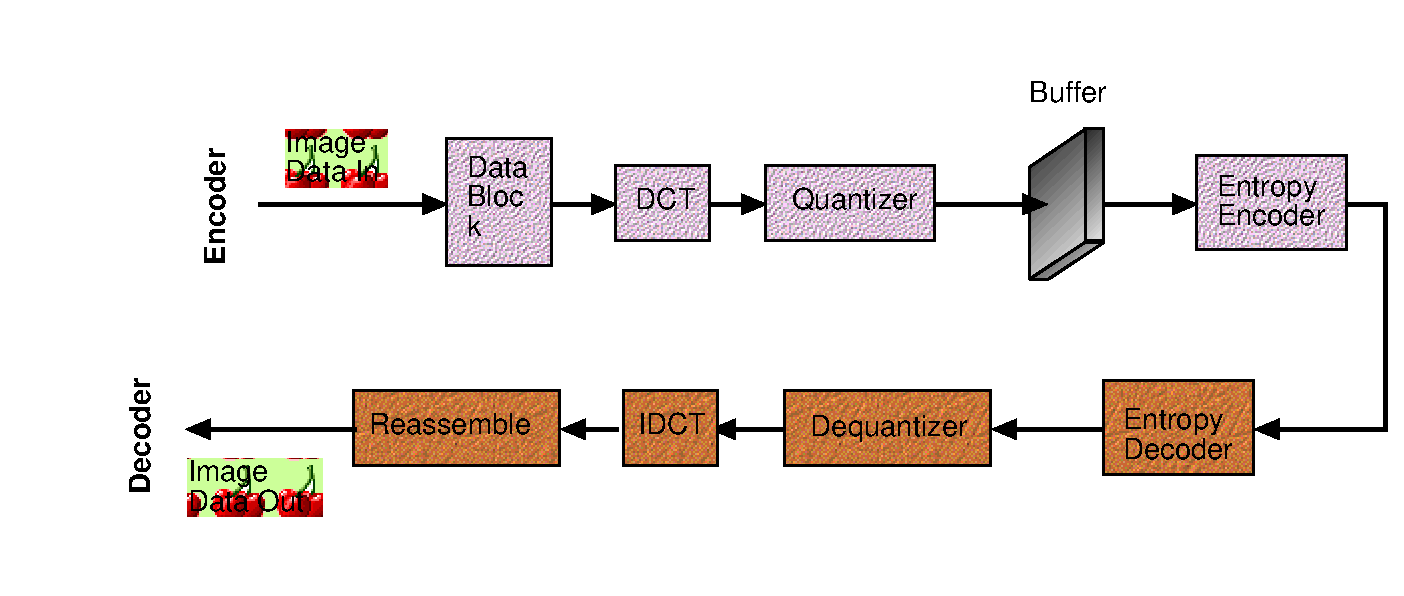
\includegraphics[width=\textwidth]{ch-av/fig9-1}}
\caption[Block diagram of JPEG encoder and decoder]{Block diagram of
JPEG encoder and decoder. The DCT, quantizer, and buffer are not used
for lossless mode. The buffer is only used for progressive
mode.\label{fg:jpeg}}
\end{figure}

Figure~\ref{fg:jpeg} presents simplified block diagrams for a JPEG
encoder and decoder.  There are four basic steps in the encoding
process:
\begin{enumerate}
\item Prepare the image data by breaking it into 8-pixel by 8-pixel
\emph{blocks}. If the image is in color, each color component (i.e.,
red, green, blue) is separately broken into blocks (in other words,
treated as though it were a separate image).

\item Decompose each block into its frequency components using the
discrete cosine transform (DCT). This is a \emph{two-dimensional} DCT, 
\index{discrete cosine transform (DCT)}
with the dimensions being the two spatial dimensions (horizontal and
vertical). Let's say we use the variable $x$ as the horizontal pixel
index and $y$ as the vertical. The location of a pixel in a block is
then $(x,y)$, where $0 \leq x \leq 7$ and $0 \leq y \leq 7$. If we use 
$p_{xy}$ to refer to the pixel \emph{value} at $(x,y)$, then the 2D
DCT of a block is
\begin{equation}
y_{kl} = \frac{c(k)c(l)}{4} \sum_{x=0}^7 \sum_{y=0}^7
           p_{xy} \cos\left[\frac{(2x+1)k\pi}{16}\right]
                  \cos\left[\frac{(2y+1)l\pi}{16}\right]
\end{equation}
where $c(k)$ and $c(l)$ are equal to $1/\sqrt{2}$ when $k$ or $l$ is
equal to zero, and 1 otherwise.

\begin{figure}
\centerline{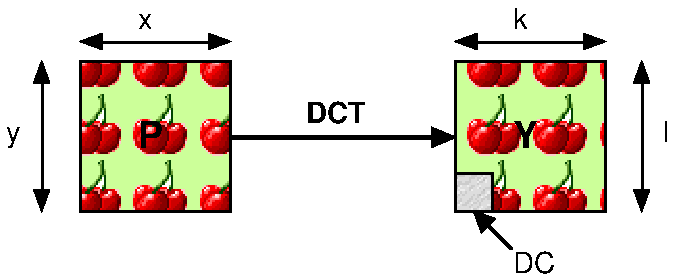
\includegraphics[width=\textwidth]{ch-av/fig9-2}}
\caption[Illustration of transform of 8x8 pixel block into 8x8 
spectrum by DCT]{Illustration of transform of 8x8 pixel block into 8x8
spectrum by DCT.  The spectrum's DC component is at $y_{00}$,
corresponding to the average intensity within the
block.\label{fg:dct}}
\end{figure}

This produces an 8x8 spectrum for the block, where frequency is in
cycles per (horizontal and vertical) pixel. The value at $y_{00}$ is
the DC value, and corresponds to the average pixel value for the
block.  Increasing $k$ and $l$ correspond to increasing spatial
frequency (more abrupt changes in image intensity). The correspondence 
between the original block and its spectrum is illustrated in
figure~\ref{fg:dct}.

\begin{figure}
\centerline{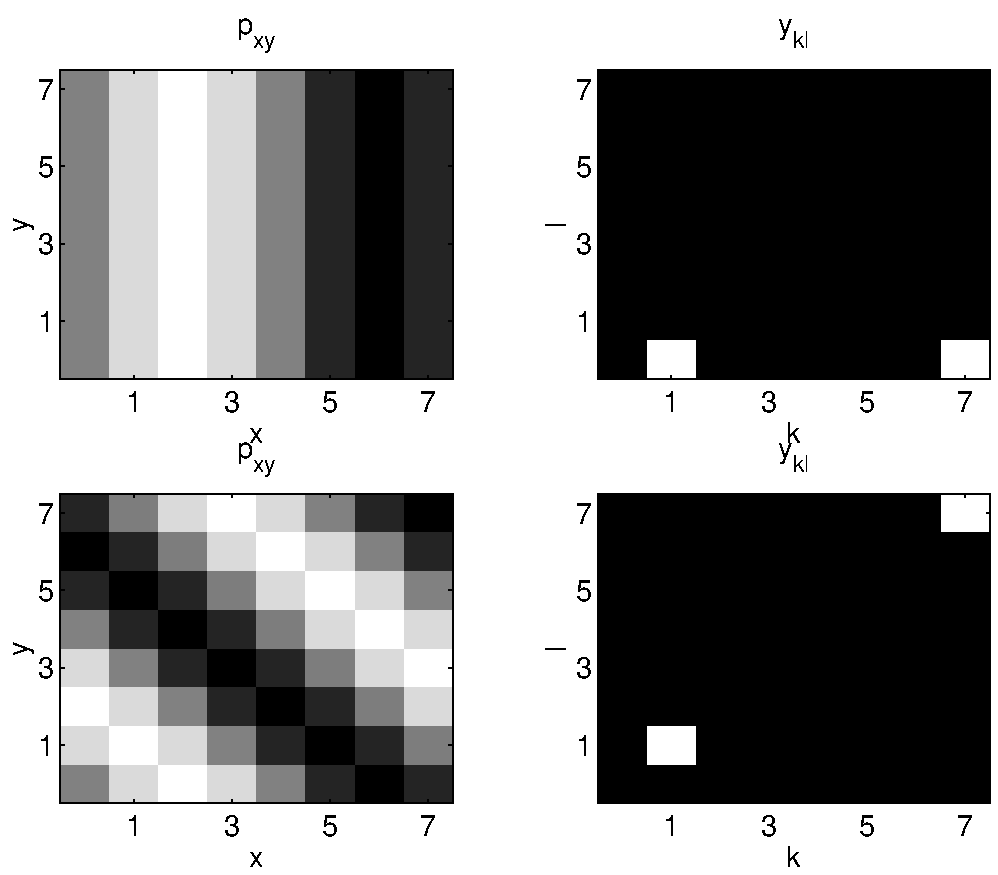
\includegraphics[width=\textwidth]{ch-av/dctdemo}}
\caption[Example 2D spectra]{Example 2D spectra. The magnitude
spectra for the 8x8 pixel blocks on the left are presented on the
right. A block with horizontal sinusoidal intensity variation at a
frequency of one cycle per 8 pixels and vertical frequency of zero
(top left) has nonzero frequency components only for $l=0$ (top
right). A block with diagonal sinusoidal intensity variation at one
cycle per 8 pixels (bottom left) has nonzero frequency components only
at some $k=l$.\label{fg:dctdemo}}
\end{figure}

Figure~\ref{fg:dctdemo} demonstrates the 2D spectra of two simple
images. In this case, the MATLAB function \verb|fft2()| was used, as
the basic MATLAB distribution has no 2D DCT built in. The resulting
complex output was converted to reals using the \verb|abs()| function
(the MATLAB code for all this is located at
\url{http://courses.washington.edu/css457/ebook/dctdemo.m}. The top
left image is a pixel block in which the pixel values vary in
intensity as the sine of the x coordinate only.  We would expect then
that it would have nonzero spectral components for $k>0$, because
there is horizontal intensity variation.  Since there is no vertical
intensity variation, the spectral components in the vertical direction
should all be zero for $l>0$. This is exactly what we see in the
spectrum plotted in the top right.

The bottom left block has sinusoidal intensity variation along
45-degree diagonals.  In this case, the rate of intensity variation is 
the same in both the $x$ and $y$ directions, so it seems logical that 
the nonzero frequency components would occur at the same horizontal
and vertical frequencies --- for $k=l$. This is shown in the plot of
the spectrum on the bottom right.

\begin{figure}
\centerline{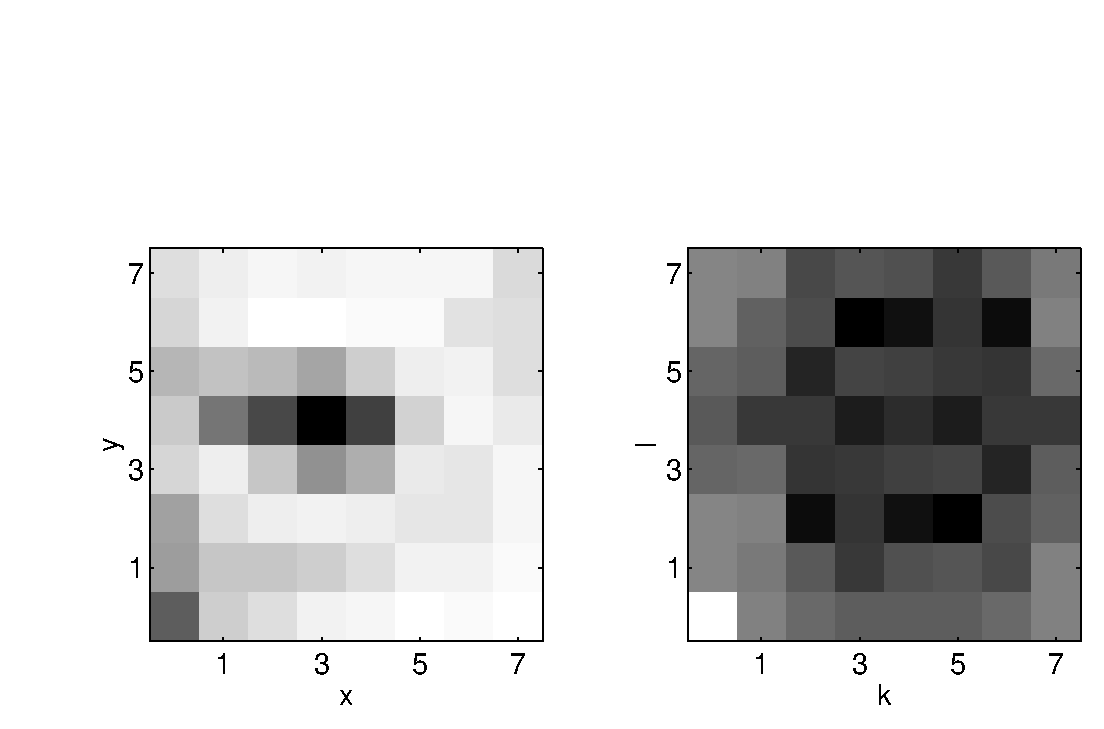
\includegraphics[width=\textwidth]{ch-av/imgdemo}}
\caption{Example spectrum (right) of an 8x8 block taken from a natural 
image.\label{fg:imgdemo}}
\end{figure}

Figure~\ref{fg:imgdemo} presents an example of the spectrum of a
natural image.  In this case, the original block (left) is someone's
eye, at fairly low resolution.  On the right in the figure, the
spectrum of the block is presented. To show the non-DC components more 
clearly, the log of the spectrum is plotted (in MATLAB,
\verb|ykl = log10(abs(fft2(pxy)));|).

\item Reduce the number of bits used to quantize each frequency
component.  An 8x8 quantization matrix, $\mathbf{Q}$, is used to
``threshold'' each element of $y_{kl}$, with the result being $z_{kl}
= \operatorname{round}(y_{kl}/q_{kl})$. Larger values for $q_{kl}$
mean that larger values for the corresponding spectral component
$y_{kl}$ will be ignored (treated as zero) and the effect is that
fewer bits will be used to quantize $y_{kl}$.  The values for
$\mathbf{Q}$ are determined by the amount of compression desired.

\begin{figure}
\centerline{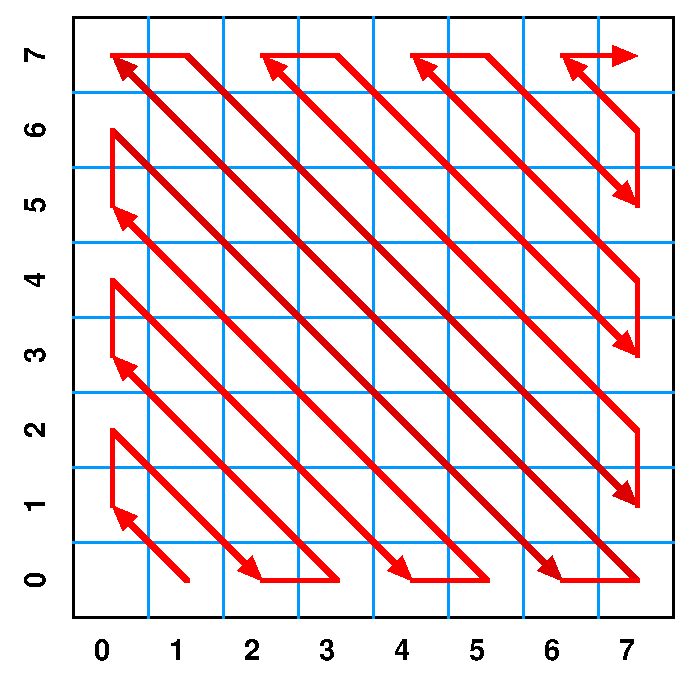
\includegraphics[width=\textwidth]{ch-av/fig9-5}}
\caption[Entropy coding of JPEG DCT blocks]{Entropy coding of JPEG DCT
blocks. Non-DC frequency components are scanned in a zig-zag
pattern.\label{fg:zigzag}}
\end{figure}

\item Perform entropy encoding. The local average brightness (the DC
component of the blocks) of images tends to vary slowly across the
image; in other words, there is a great deal of spatial redundancy in
the DC components. JPEG encodes the DC components of each block
separately (all of the DC components are encoded together).  As far as 
the other components are concerned, frequencies close to each other in 
a block tend to have the similar value.  This is especially true for
higher compression levels, where many of the high-frequency components 
will have been zeroed out.  So, the 2D DCT block is converted to a 1D
data stream by being scanned in a ``zig-zag'' pattern, as shown in
figure~\ref{fg:zigzag}.  The puts the components in increasing order
of frequency.

At this point, we have two data streams: the DC components and the
non-DC (AC) components.  The DC stream is encoded using a predictive
(difference) scheme. The AC stream is run-length coded to shrink the
runs of zero values. Then, both streams are Huffman or arithmetic
encoded.

\end{enumerate}

\section{Video Coding Standards}

Everything you've learned so far in this chapter can now be put
together, because video coding involves combining audio and multiple
still images.  The audio and image information is combined for
transmission and/or storage by \emph{multiplexing} (MUX): interleaving
\index{multiplex (MUX)}
segments of each.  On the image side of things, there's still a great
deal of redundancy in the sequence of images, because the change from
one frame of video to another is usually quite small. So, moving image
compression involves both spatial \emph{and temporal} redundancy
reduction.  There are a number of ITU standards for videoconferencing,
including H.261 and H.263. However, let's concentrate on the MPEG
standards, as they follow most directly from JPEG.

\subsection{MPEG Coding}

As MPEG-II is an extension of MPEG-I (to multiple bit rates and
resolutions), the following is applicable to both. As previously
mentioned, MPEG is a standard for video transmission and storage. It
has a higher computational complexity (on the coder side) and
bandwidth requirement (2--8Mbps) than the videoconferencing
standards. (Question: under what conditions is it acceptable to have
greater coder complexity [answer in~\ref{sc:ch9ex}
\#\ref{it:ch9ex2}]?) On the other hand, decoding has a low enough
complexity that it can be done in software.

\begin{figure}
\centerline{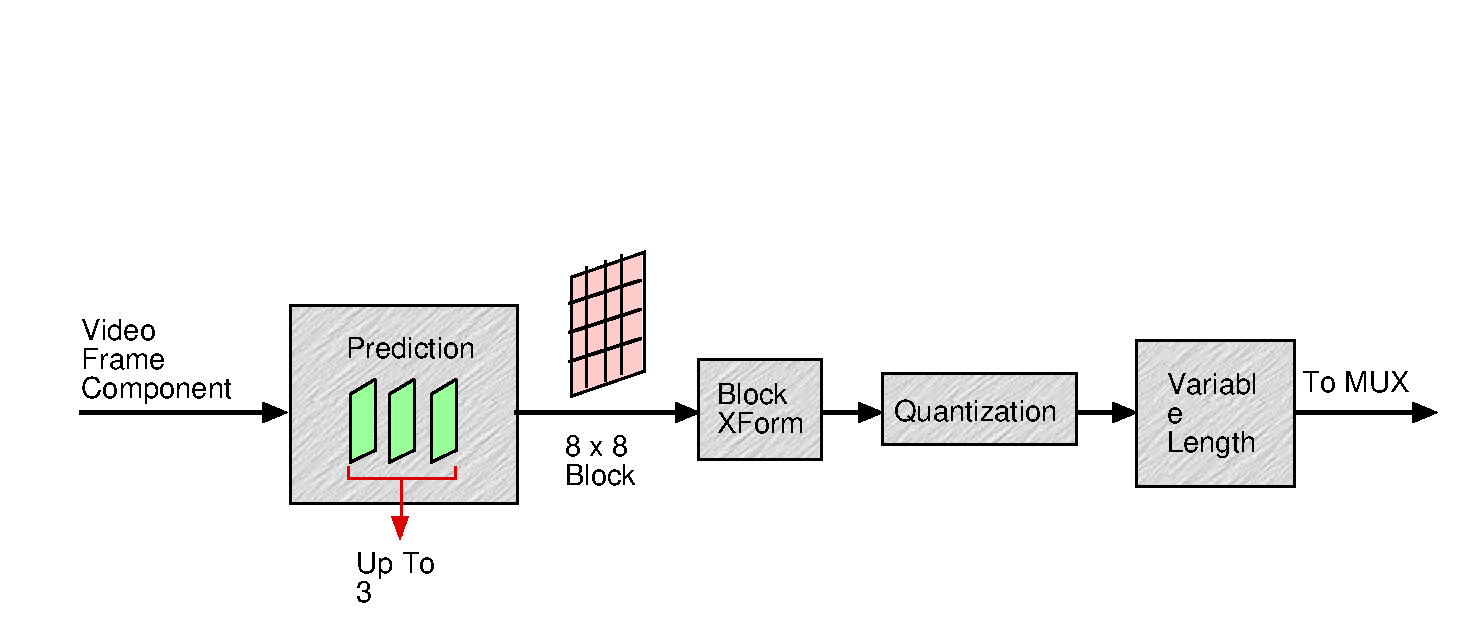
\includegraphics[width=\textwidth]{ch-av/fig9-6}}
\caption[Simplified block diagram of an MPEG video source 
encoder]{Simplified block diagram of an MPEG video source
encoder. Input frames pass through a motion compensation process, 8x8
pixel blocks are converted to a spectral representation by DCT, the
components are quantized according to the desired level of
compression, and then the result is Huffman coded.\label{fg:mpeg}}
\end{figure}

A block diagram of the MPEG coding process is presented in
figure~\ref{fg:mpeg}. Except for the ``prediction'' block and the
destination being a multiplexor, this is essentially the same as JPEG
coding.  Though it was probably implied in the discussion of JPEG that the
input could have RGB color planes, in reality MPEG color input has the
three components (Y, Cb, Cr), with the first being
\emph{luminance} (brightness) and the second and third
\emph{chrominance} (color). Because the luminance channel is more
important to our perception of visual detail, MPEG supports two
formats in which the chrominance channels have their resolutions
reduced, to either half that of luminance in both the horizontal and
vertical dimensions, or half of Y horizontally only. It is also
possible to keep all three matrices the same size. Each channel is
then processed identically, then multiplexed in the output stream.

While each input frame is structurally identical, there are three
different types of output frames:

\begin{description}
\item[I Frames] ``I,'' or \emph{intra}, frames are encoded like JPEG
images; in other words, coding only takes advantage of intra-frame
information (information within the frame). Because I frames can be
decoded in isolation, they can serve as references for random
access. A video stream in which all frames are I frames is sometimes
called \emph{MJPEG}. I frames don't use the ``prediction'' block in
figure~\ref{fg:mpeg}.
\item[P Frames] ``P,'' or \emph{predictive}, frames use the preceding
I or P frame to reduce temporal redundancy. If we ignore cuts between
scenes (where the entire image changes), changes from frame to frame
involve motion, either of the camera or of objects (or both). If we
already know what something looked like, then a simple $(x,y)$ vector
can tell where it moved to in the current frame, greatly reducing the
amount of data to send. A motion-compensation algorithm is used to
determine these motion vectors. To do this, the frame is broken into
16x16 \emph{macroblocks}. For each macroblock in the P frame, an
exhaustive search is performed in the preceding I or P frame for the
16x16 pixel region which best matches it. That area in that preceding
frame is used as a prediction for the macroblock in the current frame, 
and prediction errors and a motion vector ($(x,y)$ offset found in the
search) are computed for each 8x8 block. This corresponds to the
``prediction'' part of the block diagram, with two frames of memory
used. These errors (and motion vectors) are then sent to the block
transformation for the rest of the encoding process.
\item[B Frames] ``B,'' or \emph{bidirectional}, frames use both past
and future I and P frames for motion-compensated prediction. Two
motion vectors are computed, prediction errors are computed by
interpolating between the pixel values in the past and future frames,
and 8x8 blocks are passed to the DCT transformation process with pairs
of motion vectors.
\end{description}

An MPEG coder breaks the stream of input frames into a sequence of
GOPs, or \emph{group of pictures}.  It reorders the encoded I, P, and
B frames so that each GOP starts with an I frame and each B frame in
the GOP comes \emph{after} the two I or P frames on which it is
based. This is the best order for decoding; the decoder then converts
the frames back into display order.

The MPEG standard is not just a video or audio compression
standard. It encompasses a family of standards that include the entire 
multimedia system, including multiplexing, timing and synchronization, 
and a layered definition of the transmitted bitstream.

\section{Problems}

\begin{enumerate}
\item Discuss the decisions made with respect to the multimedia issues
described at the beginning of this chapter for MPEG-I layer 3 audio
and JPEG encoding.

\item Locate an interesting image to perform a simple test of the
effects of frequency-dependent quantization. The MATLAB image
processing or signal processing toolboxes are needed to have access to
DCT functions, so we'll use the \verb|fft2()| and \verb|ifft2()|
functions instead (if you prefer C++ or Java, then fine, but you'll
have to get hold of decent DCT implementations). The only complication 
will be the need to deal with complex numbers, mostly using the
\verb|abs()| function.
Load the image and compute its 2D FFT using \verb|fft2()| (If your
image loads as true color, with 3 color planes --- which you'll know
because its dimensions will be $N \times M \times 3$ --- then you'll
need to convert it to greyscale by adding the three components
together and dividing by 3, before computing the FFT. This can be done
by first converting it from \verb|uint8| to \verb|double| with
\verb|double|, then doing something like
\verb|a = (a(:,:,1)+a(:,:,2)+a(:,:,3)/3);|). The resulting matrix has
complex values, which we will need to preserve. Use \verb|ifft2()| to
convert the FFT back and plot the result versus the original greyscale
image (use \verb|imagesc()|) to check that everything is working fine.

Let's quantize the image's spectral content.  First, find the number
of zero elements in the FFT, using something like
\verb|length(find(a==0))|, where \verb|a| is the FFT. Next, zero out
all components with magnitudes below some threshold. You'll want to
set the threshold somewhere between the min and max magnitudes of
\verb|a|, which you can get as \verb|mn=min(min(abs(a)));| and
\verb|mx=max(max(abs(a)));|. Let's make four tests, with thresholds
5\%, 10\%, 20\%, and 50\% of the way between the min and max, i.e.,
\verb|th=0.05*(mx-mn)+mn| (you may get better results with thresholds
related to \verb|log(abs(a))|, rather than just \verb|abs(a)|). Zero
out all FFT values below the threshold using something like:
\begin{verbatim}
b = a;
b(find(abs(a)<th)) = 0;
\end{verbatim}
(substituting \verb|log(abs(a))| if that's how you're thresholding).
You can count the number of elements thresholded by finding the number 
of zero elements in \verb|b| and subtracting the number that were
originally zero. This is an estimate of the amount the image could be
compressed with an entropy coder.

Convert the thresholded FFT back to an image using something like
\verb|c = abs(ifft2(b))|. For each threshold value, plot the original
image and the processed image. You might also want to print the
difference between the two. Compute the mean squared error (MSE)
between the original and reconstructed image (mean squared error for
matrices can be computed as \verb|mean(mean((a-c).^2))|).  What can
you say about the effects on the image and MSE?  Write a script to
automate the thresholding and reconstruction, so you can easily
compute MSE for a number of thresholds. Plot MSE vs. the number of
matrix values that got thresholded?  Please submit the plots and your
code as hard copy.

\item Go through the same procedure as above, but this time, instead of 
comparing the magnitude \verb|abs(a)| to a constant, compare it to a
threshold proportional to the distance from the zero frequency (if $x$
and $y$ are subscripts to $a$, then the distance is the square root of
$x^2 + y^2$). How much more can you compress the image using this
method for the same level of MSE?
\end{enumerate}

\section{Further Reading}

\begin{itemize}
\item J. Crowcroft, M. Handley, \& I. Wakeman, \textit{Internetworking
    Multimedia}, Morgan Kaufmann, 1999, chapter~4 (\S\ 4.6--4.8,
  4.10--4.13).
\item A. Murat Tekalp, \textit{Digital Video Processing}, Prentice
  Hall, 1995, chapters 20, 23, 25.
\item K.R. Rao \& J.J. Hwang, \textit{Techniques \& Standards for
    Image, Video \& Audio Coding}, Prentice Hall, 1996, chapters
  8--12.
\end{itemize}

% LocalWords:  videoconferencing
